%!TEX root = ../../main.tex

\chapter{Theoretische Grundlagen}

\section{Unwucht}

\section{Mikrocontrollerplattform Arduino}
\textit{Arduino} ist eine aus Soft- und Hardware bestehende Plattform, dessen Komponenten nach dem Prinzip von OpenSource durch die Lizenzen \ac{LGPL} oder \ac{GPL} komplett quelloffen gehalten werden.
Die Hardware besteht aus einem E/A-Board mit aufgebrachtem Mikrocontroller und mehreren digitalen, als auch analogen Ein- und Ausgängen.
Beispielhaft ist dies in Abbildung \ref{fig:arduino_uno_schema} anhand eines Arduino UNOs dargestellt.
\begin{figure}[H]
	\centering
	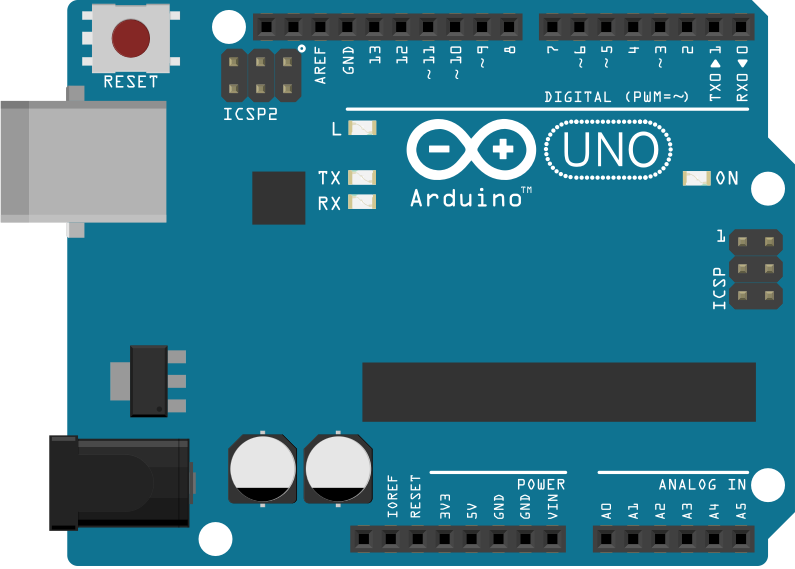
\includegraphics[width=5cm]{images/chapter/02/arduino_uno.png}
	\caption{Schamtische Darstellung eines Arduino UNOs}
	\label{fig:arduino_uno_schema}
\end{figure}
Die Boards stellen eine serielle Schnittstelle, unter anderem auch \ac{USB} zur Verfügung, über welche unter anderem die Programmierung des Mikrocontrollers stattfindet.
Die Software für den Arduino wird in einer C, bzw. C++ ähnlichen Programmiersprache geschrieben.
Für das Entwickeln des Programmes und das Programmiern des Mikrocontrollers wird von dem Hersteller eine Entwicklungsumgebung zur Verfügung gestellt, welche diese Aufgaben vereinfacht.

\begin{lstlisting}[language=C, label=arduino_sample_code, title=Beispiel-Code eines Blinklichtes für den Arduino]
int ledPin = 13;

void setup() {
    pinMode(ledPin, OUTPUT);
}

void loop() {
    digitalWrite(ledPin, HIGH);
    delay(1000);
    digitalWrite(ledPin, LOW);
    delay(1000);
}
\end{lstlisting}

Ein erfolgreiches Konzept der Arduino-Plattform sind die sogenannten \textit{Shields}.
Diese sind Zusatzleiterplatinen welche unkompliziert auf das Arduino-Board gesteckt werden und so die Funktionsvielfalt des Arduinos erweitern.
Ein besonderes Merkmal hierbei ist die Möglichkeit, dass mehrere \textit{Shields} aufeinander gesteckt werden können um so platzsparend mehrere Zusatzleiterplatinen an ein einzelnes Arduino-Board anzuschließen.
\begin{figure}[H]
	\centering
	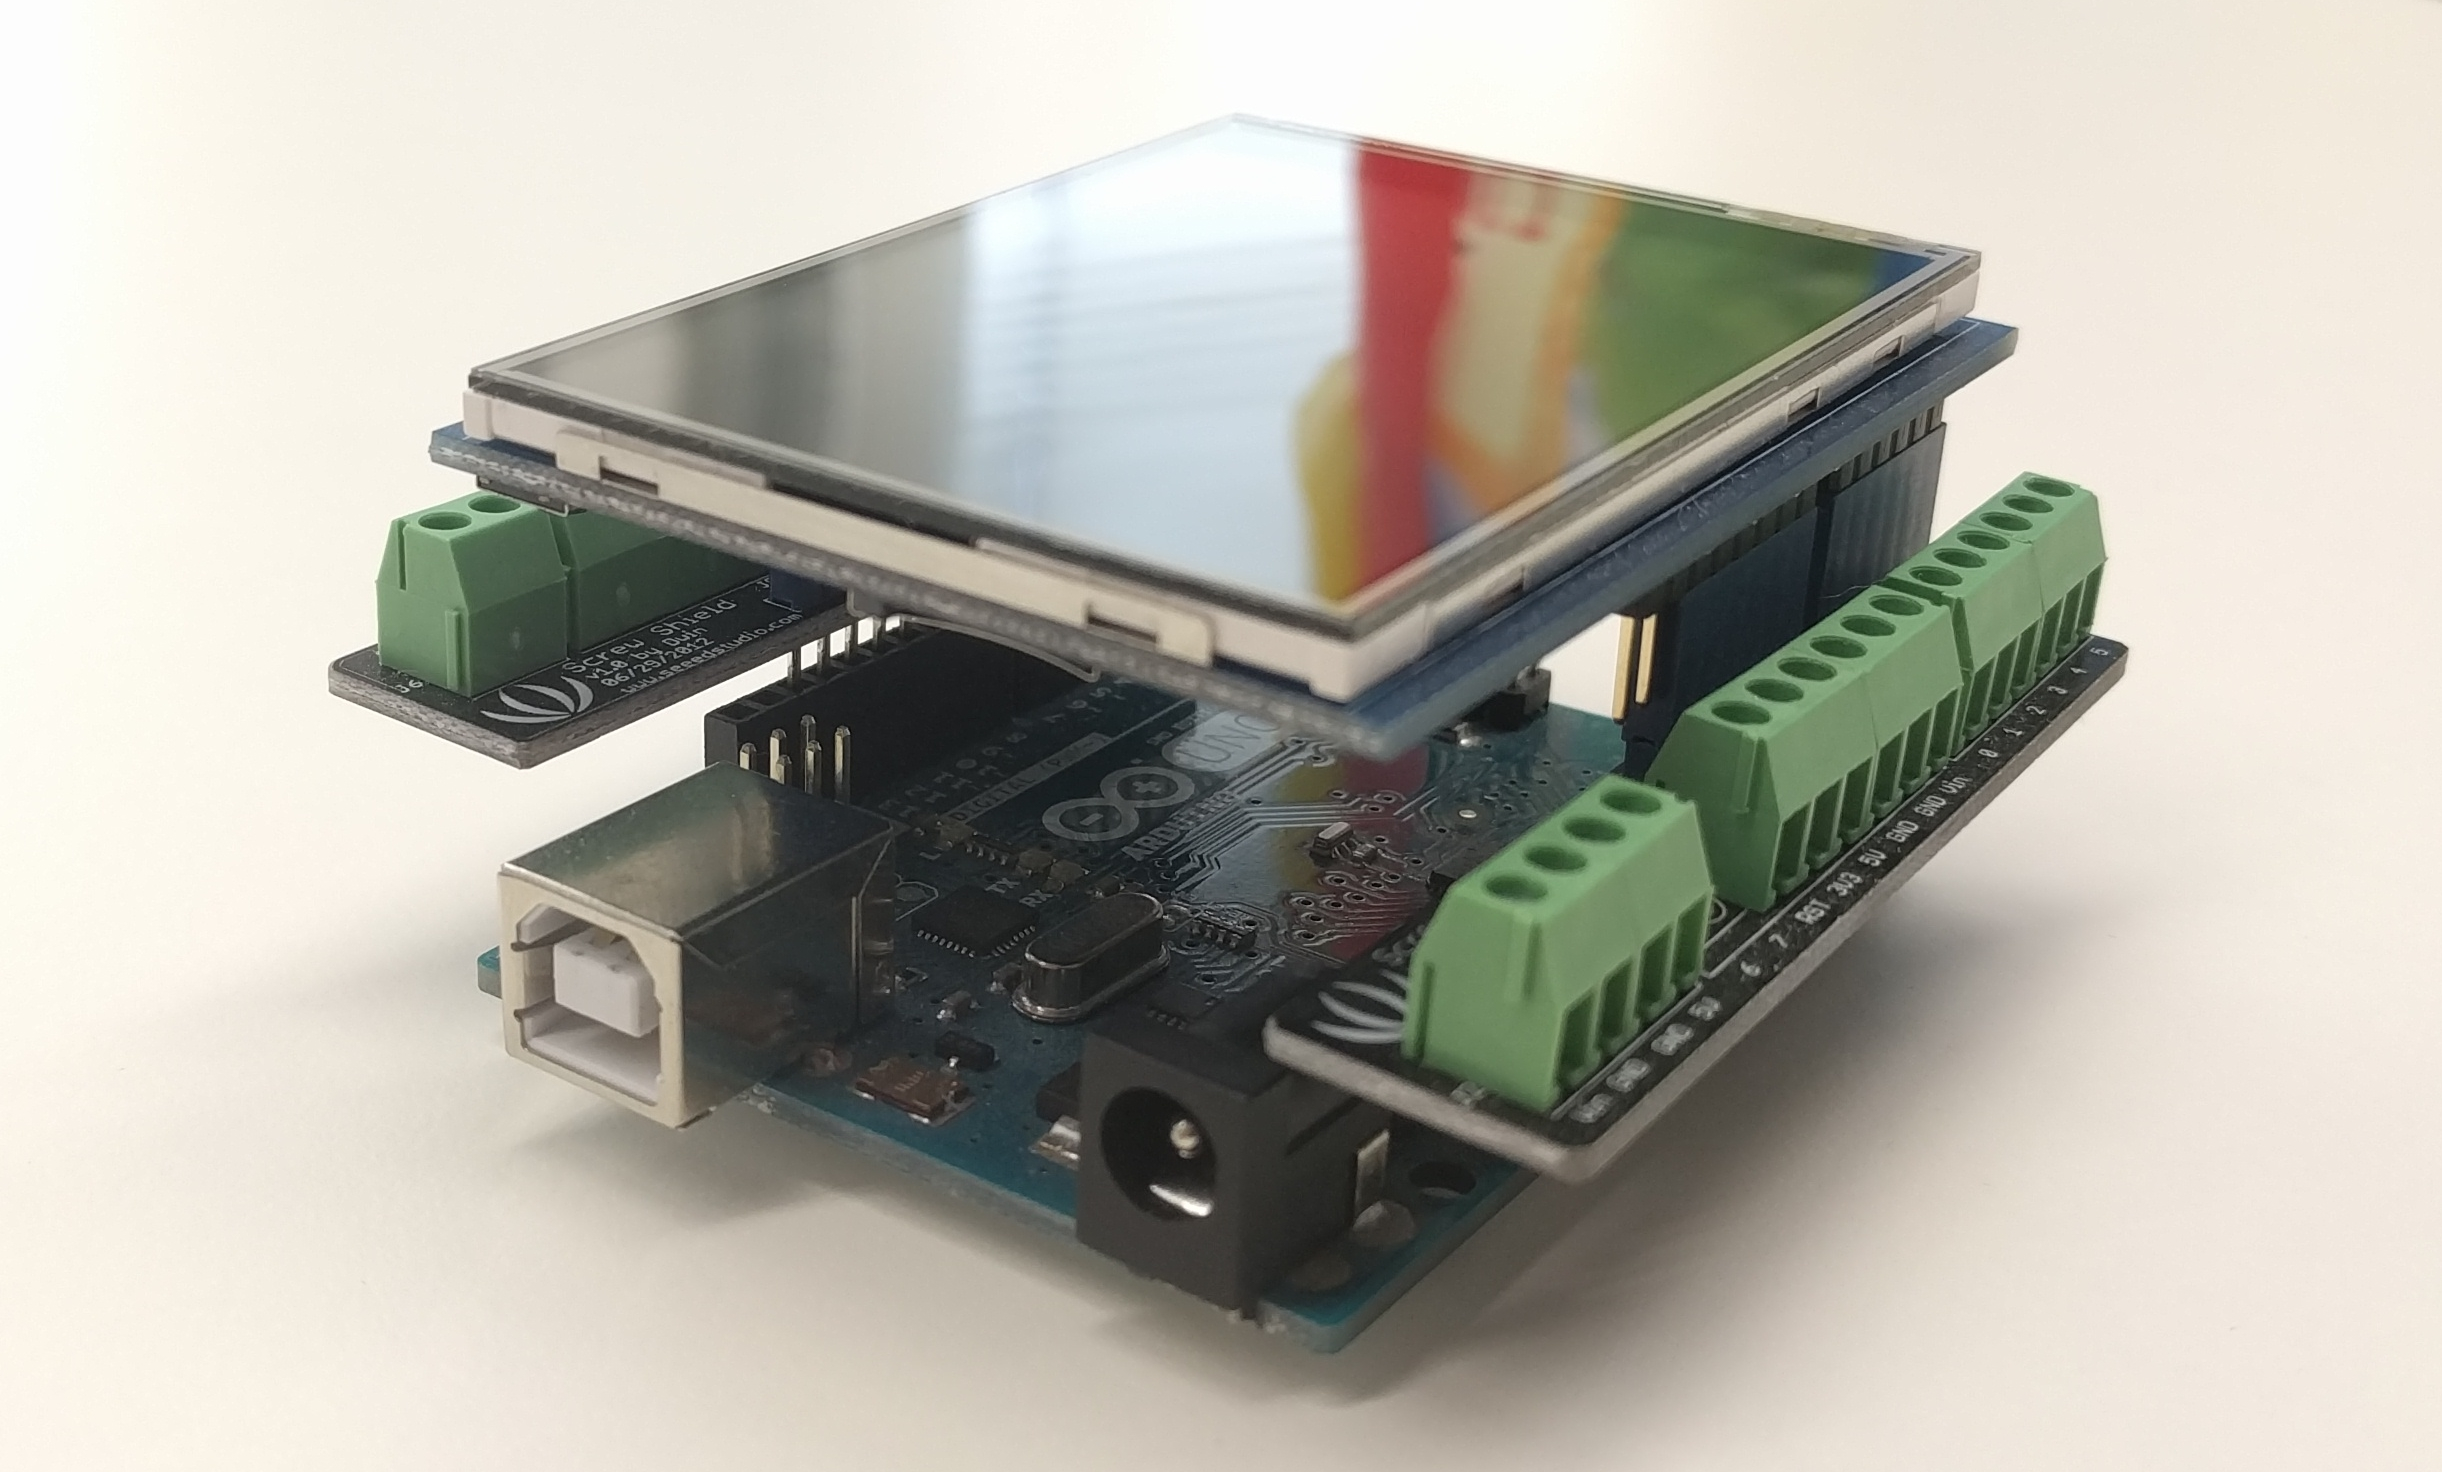
\includegraphics[width=5cm]{images/chapter/02/arduino_shields.jpg}
	\caption{Photografie eines Arduino UNOs mit zwei Shields}
	\label{fig:arduino_shield}
\end{figure}
